\documentclass[a4,12pt]{horizon-theme}
\usepackage{enumitem}

\setTitle{Detecção de Covid-19 em Radiografias do Tórax}
\setUniversity{Universidade de São Paulo}
\setFaculty{Escola Politécnica}
\setDepartment{Departamento de Eng. da Computação e Sist. Digitais}
\setCoverMainLogo{figures/minerva.pdf}

\setCoverLeftBox{%
  {\Large Projeto Final}\\[2pt]
  {PSI5790 -- Aprendizado Profundo para Visão Computacional}\\[75pt]
  {\Large Natanael Magalhães Cardoso}\\[10pt]
  {\large \textsc{nUSP:} 8914122}
}

\setCompactAuthors{Natanael Magalhães Cardoso\textsuperscript{{\large $\star$}, \faEnvelope[regular]},%
%, Prof. Cláudia Mendes de Oliveira\textsuperscript{$\dagger$}}
{ } Prof. Dr. Antonio Mauro Saraiva\textsuperscript{{\large $\star$}, $\dagger$}}

\setHeaderRight{N. M. Cardoso}
\setHeaderLeft{Escola Politécnica}

\setCompactInfo{\textsuperscript{\large $\star$} {\small Departamento de Engenharia de Computação e Sistemas Digitais, Escola Politécnica, Universidade de São Paulo.}\\[10pt]
\textsuperscript{$\dagger$} {\small Orientador}\\[10pt]
% \textsuperscript{$\dagger$} {\small Departamento de Astronomia, Instituto de Astronimia, Geofísica e Ciências Atmosféricas, Universidade de São Paulo.}\\[10pt]
\textsuperscript{\faEnvelope[regular]} {\small contato@natanael.net}\\[10pt]
{\color{gray}\rule{\linewidth}{0.4pt}}\\[10pt]
{\bf Palavras-chave:} base de conhecimento, visão computacional, vision transformers, aprendizagem profunda, busca por similaridade, astronomia extra-galática, classificação morfológica.}

\setAbstract{A astronomia produz um volume imenso de dados, principalmente na forma de imagens capturadas por telescópios e outros instrumentos. A análise dessas imagens é vital para entender o universo, descobrir novos objetos celestes e fenômenos astronômicos. Nesse sentido, este projeto aborda a aplicação de métodos de aprendizagem profunda e visão computacional na astronomia, com ênfase na análise de imagens astronômicas. O objetivo é criar um sistema inteligente que facilite descobertas astronômicas composto por um modelo de aprendizagem profunda capaz de extrair representações visuais de alta qualidade, uma base de dados para armazenar as representações obtidas e uma aplicação web para possibilidar uma exploração intuitiva de uma base dados astronômica.}



\definecolor{myred}{rgb}{0.99, 0.14, 0.12}
\newcommand{\natanael}[3]{{\fcolorbox{myred}{myred}{\color{white}Item #1:}} {\color{myred}\sout{#2}} {\color{myred} #3}}


\newcolumntype{Y}{>{\raggedleft\arraybackslash}X}
% \rowcolors{2}{blue!5!white}{blue!15!white}
\newtcolorbox[blend into=tables]{htable}[4]{%
    enhanced,
    fonttitle=\bfseries,
    colback=white,
    colframe=secondaryColor!90!white,
    colbacktitle=secondaryColor!90!white,
    coltitle=white,
    center title,
    halign title=center,
    toptitle=40pt,
    bottomtitle=40pt,
    boxrule=.8pt,
    float=!htb,
    title=\strut {#2},
    tabularx*={\arrayrulewidth0.4mm\renewcommand{\arraystretch}{1.5}}{#1},
    before upper app={#3\\\hline\hline},
    label={#4},
}


\usepackage{translator}
\usepackage{pgfgantt}
\AtBeginEnvironment{ganttchart}{\deftranslation[to=Brazilian]{May}{Mai}}
\definecolor{barblue}{RGB}{153,204,254}
\definecolor{groupblue}{RGB}{51,102,254}


\addbibresource{refs.bib}


\begin{document}
\horizonCover

% \horizonTitle

% \horizonAbstract

% \newpage
% \tableofcontents

\newpage

\onehalfspacing






\section{Introdução}
As Redes Neurais Convolucionais (CNN, \cite{lecun2015deep}), são inspiradas e propostas com certa analogia ao processamento das imagens realizadas no córtex visual de mamíferos. O processo começa quando um estímulo visual alcança a retina e equivale a um sinal que atravessa regiões específicas do cérebro. Essas regiões são responsáveis pelo reconhecimento de cada uma dessas características correspondentes \citep{karpathy2016convolutional}. De forma análoga, a CNN decompõe a tarefa de reconhecimento de um objeto em subtarefas. Para isso, a CNN divide a tarefa em subníveis de representação das características \citep{lecun2015deep}. Desta forma, as CNNs são capazes de predizer características complexas e são invariantes à escala e à rotação dos dados, o que as torna essenciais na classificação em imagens.



\section{Métodologia}
A arquitetura da rede neural convolucional projetada é esquematizada no diagrama da Fig. \ref{fig:arquitetura}. Ela é composta por camadas agrupadas em quatro blocos: pré-processamento, aumento de dados, extrator de características e camadas densamente conectadas (MLP). Cada um desses blocos serão discutidos no decorrer dessa Seção.

\begin{figure}[!ht]
  \centering
  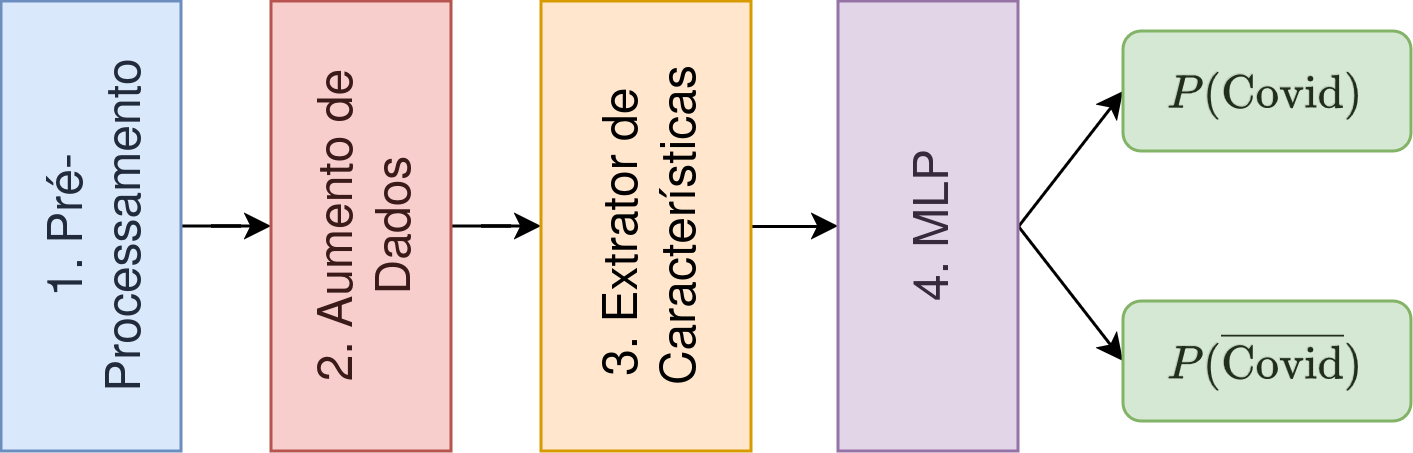
\includegraphics[width=\textwidth]{figures/diagrama-arquitetura.png}
  \caption{Arquitetura da Rede Neural, composta por camadas agrupadas em 4 blocos, pré-processamento, aumento de dados, extrator de características e camadas densamente conectadas (MLP), retornando as probabilidades para presença (ou não) de Covid-19.}
  \label{fig:arquitetura}
\end{figure}

As imagens são inicialmente carregadas como matrizes (uma única banda) de números inteiros sem sinal (unsigned int de 8 bits). O primeiro bloco, transforma as imagens em tensores de 3 bandas e aplica o pré-processamento dependendo do extrator de características utilizado. Os pixels são escalonados para o intervalo -1 a 1 para ResNet e para o intervalo 0 a 1 para as demais arquiteturas. Esses são os mesmos pré-processamentos utilizados pelos autores das arquiteturas.

O segundo bloco, é composto por camadas de aumento de dados, que poduzem transformações afins aleatoriamente nas imagens de entrada durante o treinamento. Essa técnica é utilizada para aumentar a capacidade de generalização do modelo, evitando que ele ``decore'' os padrões visuais do conjunto de treinamento. As transformações aplicadas são: espelhamento horizontal, escalonamento, variação de contraste e variação de brilho.

O terceiro bloco é composto um extrator de características, que é uma arquitetura de rede neural convolucional designada para extrair e codificar os padrões visuais da imagem de entrada. Foram selecionadas 5 arquiteturas para serem utilizadas: EfficientNet-B0 \citep{EfficientNet}, ResNet-50 \citep{ResNet},  Inception ResNet \citep{InceptionResNetv2}, DenseNet-121 e DenseNet-201 \citep{DenseNet}. A saída do extrator de característica foi reduzida aplicando \texttt{GlobalAveragePooling}, gerando um vetor unidimensional para cada exemplo do conjunto de dados. Na Seção \ref{sec:resultados}, é mostrado o desempenho de cada uma delas.

Por fim, o quarto bloco, composto por camadas densamente conectadas (\emph{Multi Layer Perceptron -- MLP}), recebem o vetor de características visuais e faz a predição final. Na última camada é usada a função \texttt{sigmoid} como ativação e nas camadas internas é usado \texttt{ReLU}. Foram utilizadas seis configurações diferentes de camadas densas: (1) uma única camada com 1024 unidades, (2) uma única camada com 512 unidades, (3) uma camada com 512 unidades seguida por outra com 256, (4) uma camada com 256 unidades seguida por outra com 256, (5) uma camada com 512 unidades seguida por outra com 512 e (6) nenhuma camada densa.



\section{Resultados e Discussão}
\label{sec:resultados}
Inicialmente, foram testadas combinações das arquiteturas selecionadas com configurações de blocos MLP. A Fig. \ref{fig:model_arch} mostra o desempenho dos modelos treinados no conjunto de validação agregados por arquitetura. Tanto para inicialização aleatória, quanto para inicialização com pré-treino na Imagenet, a arquitetura EfficientNet B0 superou as demais e, portanto, as análises seguintes refem-se ao modelo utilizando esta arquitetura.

\begin{figure}[!ht]
  \centering
  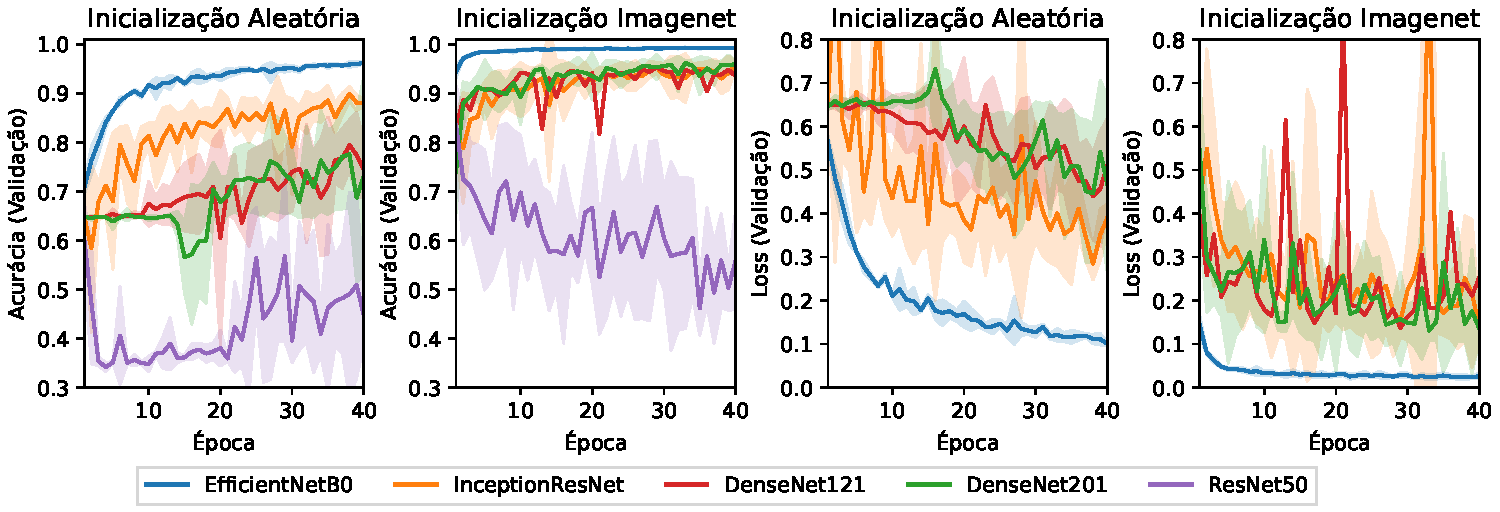
\includegraphics[width=\textwidth]{figures/model_arch.pdf}
  \caption{Desempenho de várias arquiteturas convolucionais no conjunto de validação. Da esquerda para direita, os painéis mostram os valores de acurácia e da função de custo para inicialização aleatória e transferência de aprendizagem a partir de um modelo treinado na Imagenet. A área sombreada representa um desvio padrão.}
  \label{fig:model_arch}
\end{figure}

\newpage
Após avaliar os modelos, o que possuiu menor loss no conjunto de validação foi escolhido. Para ambos os casos (inicialização aleatória ou por transferência de aprendizagem), o melhor resultado foi obtido sem utilizar camdas ocultas no bloco MLP. Os modelos foram treinados com otimizador Adam inicializado com taxa de aprendizagem $4\times 10^{-5}$.

% Além disso, como o conjunto de dados é moderadamente desbalanceado, foi utilizada a técnica de ponderamento de classes (atribuição de pesos para cada classe no cálculo da função de custo). Para o modelo pré-treinado com Imagenet, esta técnica não teve impacto na melhora da avaliação. No entanto, para o modelo treinado com inicialização aleatória, esta técnica melhorou o desempenho do modelo.
A avaliação do modelo no conjunto de teste se deu pela análise da curva ROC e das matrizes de confusão. É notável que o modelo pré-treinado na Imagenet possui maior capacidade preditiva do que o treinado com inicialização aleatória dos pesos. Os valores da área abaixo da curva ROC obtidos foram 0.9924487 e 0.9999885 para inicialização aleatória e transferência de aprendizagem, respectivamente, que no gráfico, foram arredondados para 1

\begin{figure}[!ht]
  \centering
  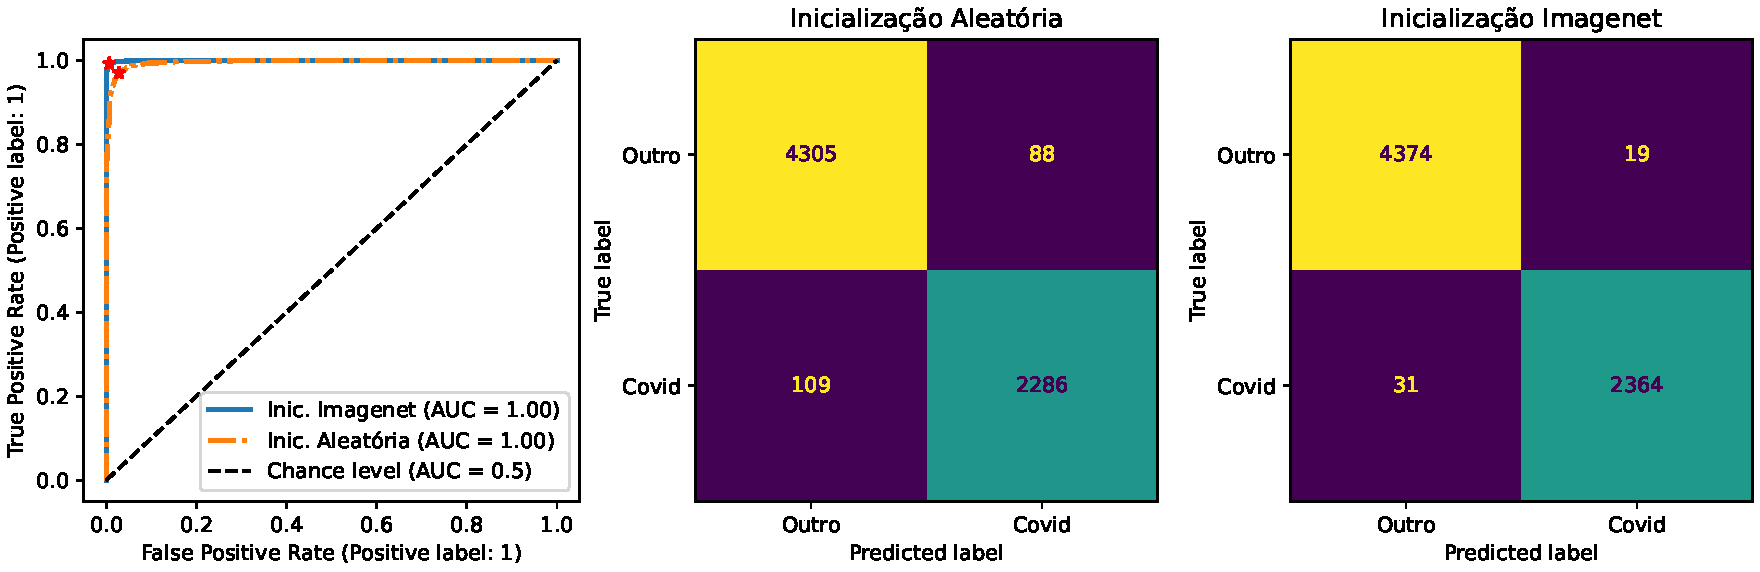
\includegraphics[width=\textwidth]{figures/best_models_cm.pdf}
  \caption{Da esquerda para direita: curvas ROC e matrizes de confusão para modelo pré-treinado e inicialização aleatória, respectivamente.}
  \label{fig:x}
\end{figure}


% \begin{figure}[!ht]
%   \centering
%   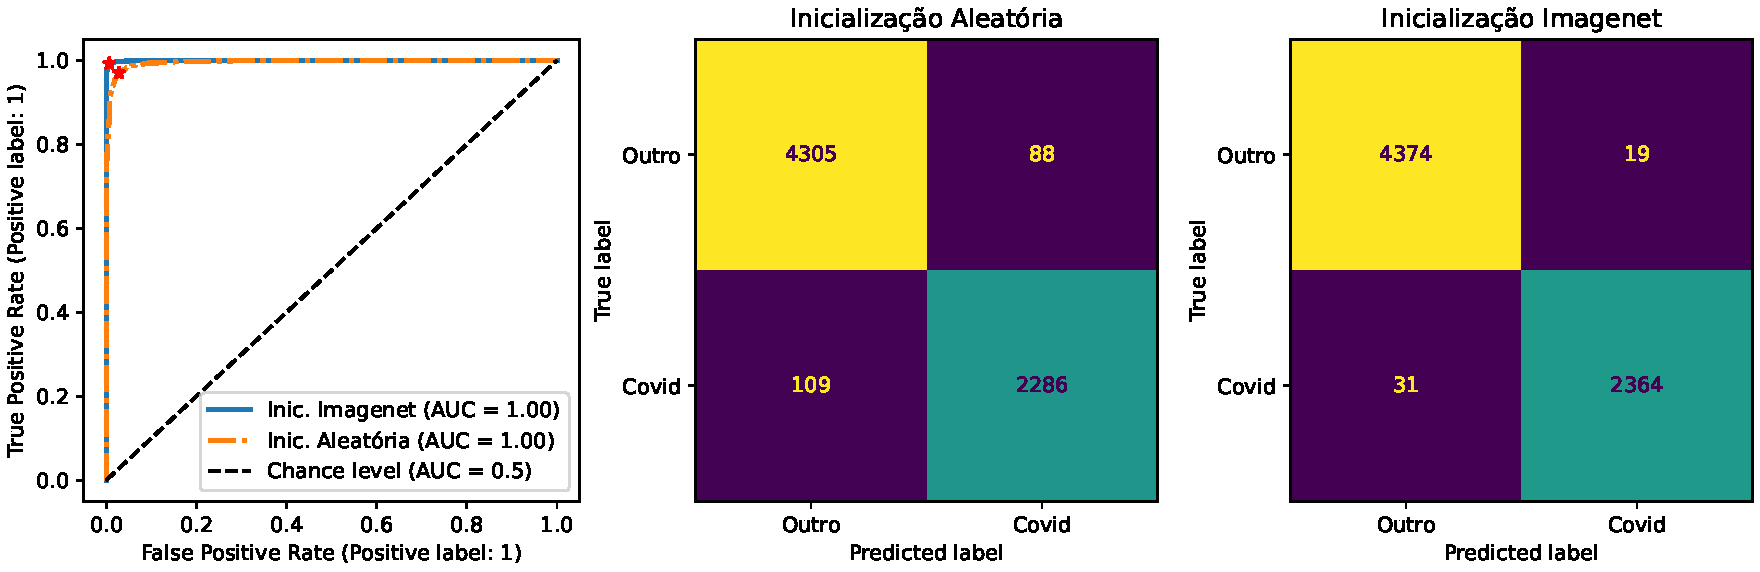
\includegraphics[width=\textwidth]{figures/best_models_cm.pdf}
%   \caption{Matriz de confução para o melhor modelo treinado com inicialização aleatória (esqueda) e por transferência de aprendizagem (direita).}
%   \label{fig:cm}
% \end{figure}


\section{Conclusão}
Neste estudo, foi feita uma análise comparativa do impacto da técnica de transferência de aprendizagem para inicialização dos pesos em uma rede neural convolucional pré-treinada na Imagenet. Ao avaliar os modelos no conjuto de teste usando as cuvas ROC e a matriz de confusão, foi constado que esta técnica garante um aumento significativo na capacidade preditiva do modelo, como discutido na avaliação

Assim, a partir deste estudo, conclui-se que é possível treinar um modelo de alta capacidade preditiva para Covid-19 utilizando redes neurais convolucionais pré-treinadas na Imagenet


\printbibliography


\horizonBackCover
\end{document}
